% !TeX root = ../translation.tex

\section{计算算法}

 Brenier定理可以直接推广到离散的情况下。在GAN模型中,源测度$\mu$被定义为紧凸域$\Omega$上的均匀(或高斯)分布;目标测度$\nu$表示为经验测度,它是狄拉克测度的和:
\begin{equation}
	\nu = \sum_{i=1}^{n} \nu _i \delta (y-y_i)
	\label{function:17}
\end{equation}
其中,$Y=\{ y_1, y_2, \cdots, y_n \}$为训练样本,具有权重:$\sum_{i=1}^{n} \nu _i=\mu(\Omega)$;$\delta$为特征函数。

每个训练样本$y_i$对应于 Brenier势的一个支撑平面,表示如下:
\begin{equation}
	\pi _{h,i} (x) =\left \langle x , y_i \right \rangle +h_i 
	\label{function:18}
\end{equation}
其中,支撑平面的截距(高度)$h_i$是一个未知的变量。我们将所有的高度变量表示为$h=(h_1,h_2,\cdots ,h_n)$。

欧几里得空间中一族超平面的包络是一个超曲面,它在某一点上与族的每个成员相切,这些切点一起构成了整个包络。如图 \ref{fig:6} 所示,Brenier势$u_h : \Omega \to \mathbb{R}$是一个由$h$决定的分段线性凸函数,它是其所有支撑平面的上包络线:
\begin{equation}
	u_h(x)=\max_{i=1}^{n}\left [ \pi _{h,i}(x) \right ] =\max_{i=1}^{n}\left [ \left \langle x,y_i \right \rangle +h_i \right ]
	\label{function:19}
\end{equation}

\begin{figure}[h]
	\centering
	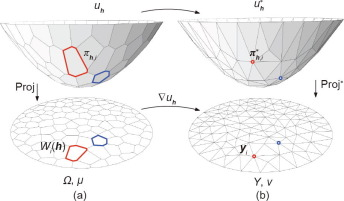
\includegraphics[width=0.6\linewidth]{6.jpg}
	\caption{分片线性Brenier势能函数(a)及其Legendre变换$u_h^*(b)$。$\pi_{h,n}^*$;$\pi_{h,i}$的Legendre对偶;$\bigtriangledown  : u_k$的梯度;Proj:投影映射;Proj*:Legendre对偶空间内的投影映射。}
	\label{fig:6}
\end{figure}

Brenier势能图是一个凸多面体。每个支撑平面$\pi_{h,i}$,i对应于多面体的一个面。多面体的投影诱导了$\Omega$的胞腔分解,其中每个支撑平面$\pi _i(x)$投射到一个胞胞$W_i(h),p$上是$\mathbb{R}^d$中的任意点:
\begin{equation}
	\Omega=\bigcup_{i=1}^{n} w_i(h) \cap \Omega, W_i(h)=\left \{ p \in \mathbb{R}^d \mid \bigtriangledown  u_h(p)=y_i \right \}  
	\label{function:20}
\end{equation}

胞腔分解是一个功率图。$W_i \cap \Omega$的$\mu$-测度记为$w_i(h)$:
\begin{equation}
	w_i(h)=\mu\left [ W_i(h) \cap \Omega \right ] = \int _{W_i(h) \cap \Omega}\mathrm{d}\mu  
	\label{function:21}
\end{equation}

梯度映射:$\bigtriangledown u_h : \Omega \to Y$将每个单元格$W_i(h)$映射到一个点$y_i$:
\begin{equation}
	\bigtriangledown u_h : W_i(h) \to y_i, i=1,2, \cdots ,n 
	\label{function:22}
\end{equation}

给定等式(\ref{function:17})中的目标度量$\nu$,在等式(\ref{function:19})中存在一个离散的布雷尼尔势,其每个面$w_i(h)$的投影$\mu$体积等于给定的目标度量$\nu _i$。 Alexandrov[46]在凸几何中证明了这一点。
\begin{theorem}[Alexandrov【46】] \label{theorem:4.1}
	假设$\Omega$是一个紧凑的凸多面体,在$\mathbb{R}^d$中内部为非空,$n_1,\cdots, n_k \subset \mathbb{R}^{n+1}$是不同的$k$个单位向量,$(n+1)$坐标为负,$v_1,\cdots, v_k > 0$,因此$\sum_{i=1}^{k} \nu _i= vol(\Omega)$ 。然后存在一个有精确$k$余维-1面$F_1, \cdots ,F_k$的凸多面体$P \subset \mathbb{R}^{n+1}$,其中$n_i$是$F_i$的法向量,并且在$\Omega$和$F_i$的投影之间有体积$v_i$。此外,这种$P$在垂直平移之前是唯一的。
	
	Alexandrov的解的存在性证明是基于代数拓扑,这不是构造性的。最近,Gu等人[6]提供了一个基于变分方法的构造性证明。
\end{theorem}

\begin{theorem}[参考文献【6】]\label{theorem:4.2}
	设$\mu$是定义在$\mathbb{R}^d$紧凸域$\Omega$上的概率测度,设$Y=\{ y_1,y_2,\cdots, y_n \}$是$\mathbb{R}^d$中的一个不同点。然后对于$\sum_{i=1}^n v_i=\mu(\Omega)$的任何$v_1,v_2,\cdots, v_n>0$,对于所有$i$,存在唯一的添加一个常数$(c,c,\cdots,c)$使得$w_i(h)=v_i$的$h=(h_1,h_2,\cdots, h_n)\in \mathbb{R}^n$。向量$\mathbf{h}$是以下凸能量的唯一最小值参数:
	\begin{equation}
		E(h) =\int_0^h \sum_{i=1}^n w_i(\eta)\mathrm{d}\eta_i  - \sum_{i=1}^n h_iv_i
		\label{function:23}
	\end{equation}

	定义在一个开的凸集上
	\begin{equation}
		H=\left \{ h\in \mathbb{R}^d : w_i(h)>0,i=1,2,\cdots ,n  \right \} 
		\label{function:24}
	\end{equation}

	此外,$\bigtriangledown u_k$使二次代价最小化
	\begin{equation}
		\frac{1}{2} \int_{\Omega} \left \| x-T(x) \right \|^2 \mathrm{d}\mu(x)
		\label{function:25}
	\end{equation}
	在所有的传输映射中,$T_{\# \mu} = \nu$。
	
	上述凸能量在等式(\ref{function:23})中的梯度值如下:
	\begin{equation}
		\bigtriangledown E(h)=\left [ w_1(h)-v_1, w_2(h)-v_2, \cdots , w_n(h)-v_n \right ]^T
		\label{function:26}
	\end{equation}

	能量的第$i$行和第$j$列元素如下:
	\begin{equation}
		\frac{\partial w_i}{\partial h_j} =-\frac{\mu (W_i \cap W_j \cap \Omega)}{\left \| y_i-y_j \right \| }, \frac{\partial w_i}{\partial h_i} = \sum_{j\ne i}\frac{\partial w_i}{\partial h_j} 
		\label{function:27}
	\end{equation}

	如图 \ref{fig:6} 所示,Hessian矩阵有一个明确的几何解释。图\ref{fig:6}(a)显示了离散的布雷尼尔势$u_h$,而图\ref{fig:6}(b)显示了其使用定义(\ref{definition:3.3})的勒让德变换。勒让德变换可以用几何方法构造:对于每个支撑平面$\pi_{h,i}$,我们构造对偶点$\pi_{h,i}^*$;对偶点的凸包$\{\pi_{h,1}^* ,\pi_{h,2}^* , \cdots , \pi_{h,n}^* \}$是勒让德变换的图$u_h^*$。
	
	$u_h^*$的投影得到了一个的三角剖分$Y=\{ y_1,y_2, \cdots ,y_n \}$,即加权的德劳内三角剖分。如图\ref{fig:7}所示,等式(\ref{function:20})中的能量图和加权的德劳内三角剖分是庞加莱对偶的:如果在幂图中,$W_i(h)$和$W_j(h)$在一个$(d-1)$-维胞腔上相交,那么在加权的德劳内三角剖分中,$y_i$与$y_j$连接。在等式(\ref{function:27})中的黑森矩阵的元素是能量图中$(d-1)$单元的$\mu$体积与加权德劳内三角剖分中双边的长度之间的比值。
\end{theorem}

传统的幂次图可以与上述定理密切相关。

\begin{figure}[h]
	\centering
	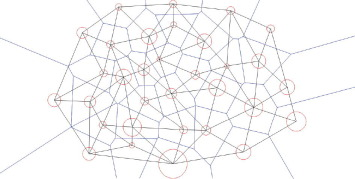
\includegraphics[width=0.6\linewidth]{7.jpg}
	\caption{Power diagram(蓝色)和其对偶加权Delaunay三角剖分(黑色)。}
	\label{fig:7}
\end{figure}


\begin{definition}[power距离]\label{definition:4.1}
	给定一个功率权重为$\psi _i$的点$y_i \in \mathbb{R}^d$,power距离如下:
	\begin{equation}
		pow(x,y_i)=\left \| x-y_i \right \|^2 -\psi _i
		\label{function:28}
	\end{equation}
\end{definition}

\begin{definition}[power图]\label{definition:4.2}
	给定加权点$(y_1,\psi _1), \cdots , (y_k, \psi _k)$,幂图为单元分解的$\mathbb{R}^d$:
	\begin{equation}
		\mathbb{R}^d=\bigcup_{i=1}^{k} W_i(\psi) 
		\label{function:29}
	\end{equation}
	其中,每个单元格都是一个凸多面体:
	\begin{equation}
		W_i(\psi)=\left \{ x \in \mathbb{R}^d \mid pow(x,y_j) \le pow(x,y_j) \right \} 
		\label{function:30}
	\end{equation}
	
	加权德劳内三角剖分,记为$T(\psi)$,是幂图的庞加莱对偶;如果$W_i(\psi)\cap W_j(\psi) \ne \phi$,那么在加权德劳内三角剖分中有一条边连接$y_i$和$y_j$。注意,$pow(x,y_i) \le pow(x,y_j)$等价于
	\begin{equation}
		\left \langle x,y_i \right \rangle +\frac{1}{2} (\psi _i -\left \| y_i \right \|^2 ) \ge \left \langle x,y_j \right \rangle + \frac{1}{2} (\psi _j -\left \| y_j \right \|^2 )
		\label{function:31}
	\end{equation}

	让$h_i=\frac{1}{2} (\psi _i - \left \| y_i \right \|^2 )$;然后我们将其定义重写如下:
	\begin{equation}
		W_i(\psi)=\left \{ x \in \mathbb{R}^d \mid \left \langle x,y_i \right \rangle +h_i \ge \left \langle x,y_j \right \rangle +h_j , \forall j \right \} 
		\label{function:32}
	\end{equation}
\end{definition}

在实践中,我们的目标是计算离散的布雷尼尔的潜在等式(\ref{function:19})通过优化凸能量等式(\ref{function:23}).对于低维情况,我们可以通过计算牛顿方法直接计算梯度等式(\ref{function:26})和黑森矩阵等式(\ref{function:27})。对于深度学习应用,直接计算黑森矩阵是不可行的;相反,我们可以使用梯度下降法或具有超线性收敛性的拟牛顿法。梯度的关键是估计$\mu$体积$w_i(h)$。这可以用蒙特卡罗方法来实现:我们从分布$µ$中抽取$n$个随机样本,并计算在$W_i(h)$范围内的样本数量,这是收敛于$\mu$体积的比值。这种方法是纯并行的,可以使用GPU来实现。此外,我们还可以使用分层的方法来进一步提高效率:首先,我们将目标样本分类为聚类,并计算到聚类质量中心的OT映射;其次,对于每个聚类,我们计算从相应的细胞到聚类内原始目标样本的OT映射。

\begin{figure}[h]
	\centering
	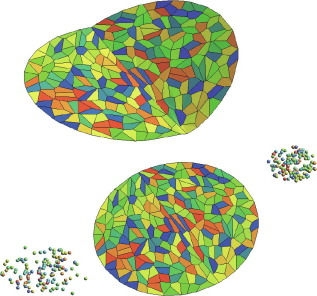
\includegraphics[width=0.6\linewidth]{8.jpg}
	\caption{Brenier势能函数的奇异点集与OT映射的间断点集。}
	\label{fig:8}
\end{figure}

为了避免模态坍塌,我们需要在$\Omega$中找到奇异点集。如图\ref{fig:8}所示,目标狄拉克测度有两个簇;源是单位平面圆盘上的均匀分布。布雷尼尔势函数的图是一个中间有一个脊的凸多面体。脊在圆盘上的投影是奇异集$\sum_1(u)$,最优映射在$\sum_1$上是不连续的。在一般情况下,如果两个单元格$W_i(h)$和$W_j(h)$相邻,则我们计算法线与相应支撑平面之间的夹角:
\begin{equation*}
	\theta _{ij} =\frac{\left \langle x_i,y_j \right \rangle }{\left \| y_i \right \| \left \| y_j \right \| } 
\end{equation*}

如果$\theta _{ij}$大于一个阈值,则公共面$W_i(h) \cap W_j(h)$在不连续奇异集合中。